%!TEX root = ../LastNameI-[RnD-MT]Report.tex
\chapter{Experimental Evaluation \& Results}
\label{ER}
This chapter presents experiments performed to evaluate and analyze on the \textit{proof of concept implementation} given to the extension of Popov Vereshchagin solver. The evaluation gives theoretical and practical explanation to the hypothesis which has been discussed in chapter \ref{Approach}. The chapter begins by discussing over evaluation on singularities and then providing a comparison between  run time complexities of decomposition techniques by benchmarking them.
\section{Experimental setup}
All of the tests were conducted in simulation environment. The test setup created to show the equivalence between implemented approach of detecting the singularities within the solver and the traditional (ground truth) singularities. Different scenarios have been evaluated, firstly in-order to find the equivalence between the traditional singularities and the dynamic singularities detected. Later on to test by randomizing input task constraints on the end effector, to check if task constraints are satisfiable in the kinematic chain. The main reason for conducting the experiments is to give a validation for the proposed approach in chapter \ref{Approach}.


For the conducted experiments, the design of the robot model follows the specifications of KUKA LWR. Mass of each segment is 2 \textit{kg} and the joint specifications and frame assignment follow the model specified in OROCOS KDL. The model is also maintained to not compensate for gravity effects. Also mainly for the experimentation, giving the end effector with different task constraints specifications and joint specifications, we try to validate the results if they indicate the cases with singularity and their correctness of measurement. 
%There are two major scenarios which have been evaluated, i.e.\ modeling of kinematic chain when being configured in singular configuration. 
\section{Test scenarios}
%For the first experimentation the end effector has been constrained completely. 
%The kinematic chain has been modeled to be in stretched out configuration (see figure \ref{}) \
In the first scenario, the KUKA-LWR (7R manipulator) is explicitly maintained in different singular configurations . The first configuration of the manipulator is completely extended (see figure \ref{singular1}), with zero joint configuration ($q=0$) for all the joints. The end effector is completely constrained for this case. This indicates that the arm is in singular configuration and cannot achieve all the task constraints as specified in the end effector as some of the joints are restricted. Similarly, the second singular configuration can be seen in figure \ref{singular2} as the manipulator loses few DOF's.
%	\begin{figure}[h!]
%		\centering
%		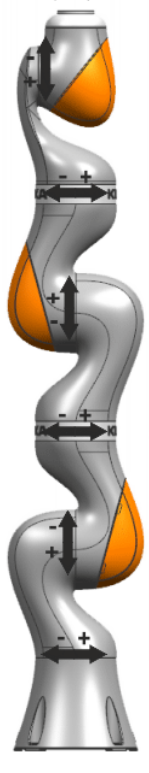
\includegraphics[width=0.08\textwidth]{images/kuka}
%		\caption{7R manipulator in completely extended configuration}
%		\label{kuka}
%	\end{figure}


In the second case, the input joint configurations are randomized along with end effector Cartesian acceleration constraints. These cases validated for random joint configurations as seen in figures \ref{nonsingular1} and \ref{nonsingular2}. The main intention behind this test case, is to provide validation of the derived approach to check if it is able to detect singularities and able to perform separation of concerns between detection of singularity and providing decision of exploiting this knowledge to others (decision making refer \ref{Controlscheme2}). This setup is also mainly developed to check if all the task constraints applied are satisfiable and if they are detected within the sweeps. 
% This indicates that the manipulator is in singular configuration (boundary singularity).

\section{Results and Discussions}
The results in the first case indicated that certain task constraints are satisfied while some of them cannot. This specifies that the kinematic chain is in singular configuration and some of the joints are restricted. In case of figure \ref{singular1} the algorithm validates that the task constraint can be satisfied linearly in \textit{x} directions and angularly in \textit{y} and \textit{z} directions which complement the physical interpretations. However, to match the findings in Popov Vereshchagin solver to traditional singularity, the rank of the constraint coupling matrix is determined and compared to the rank of Jacobian. The results indicate that they are equivalent. Similarly the result of other configuration in singularity (see figure \ref{singular2}) also indicated that all the end effector constraints are not satisfiable and task specification in linear \textit{z} direction is not achievable.

The results for the second scenario indicated that all the task constraints are achievable and the kinematic chain is not in singularity.


\begin{figure}[h!]
		\begin{minipage}{0.35\textwidth}
			\centering
			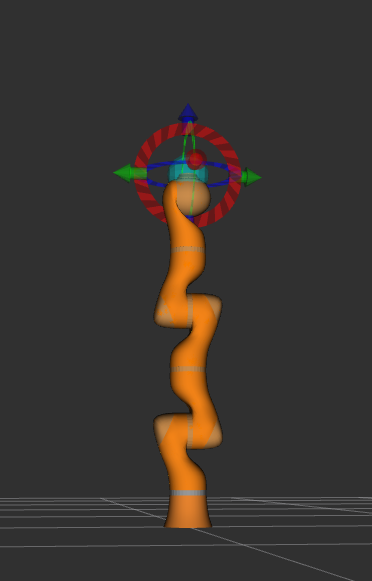
\includegraphics[width=5.5cm,height=6cm]{images/kukaconfiguration3}
			\caption{Arm in home configuration}
			\label{singular1}
		\end{minipage}\hfill
			\begin{minipage}{0.35\textwidth}
				\centering
				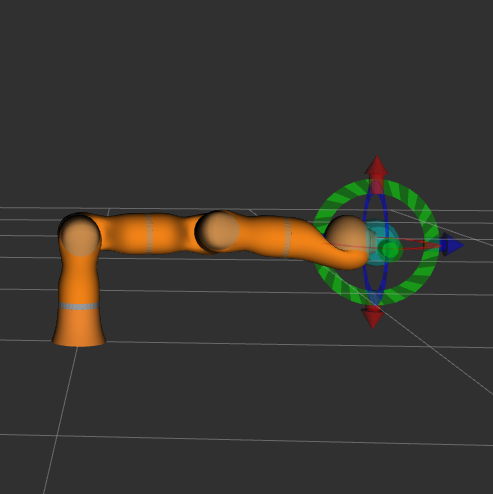
\includegraphics[scale=0.34]{images/kukac4}
				\caption{Arm in singular configuration}
				\label{singular2}
			\end{minipage}
\end{figure} 
\begin{figure}[h!]
	\centering
	\begin{minipage}{0.35\textwidth}
		\centering
		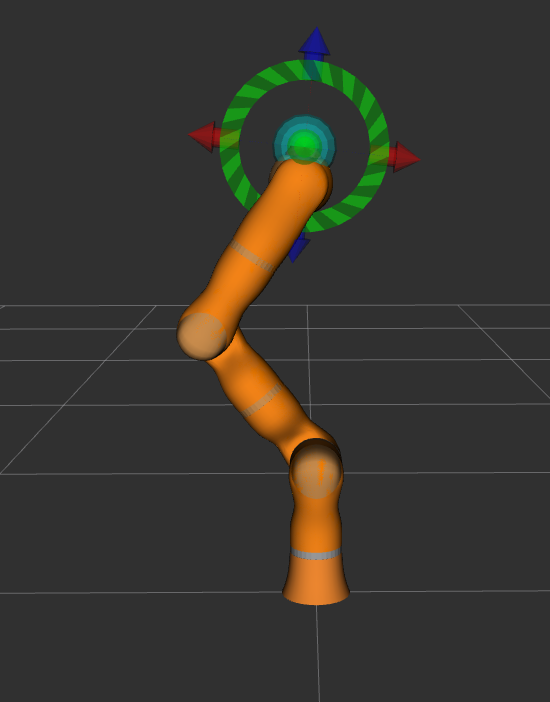
\includegraphics[scale=0.25]{images/kukaconfiguration1}
		\caption{Arm in non singular configuration}
		\label{nonsingular1}
	\end{minipage}\hfill
	\begin{minipage}{0.35\textwidth}
		\centering
		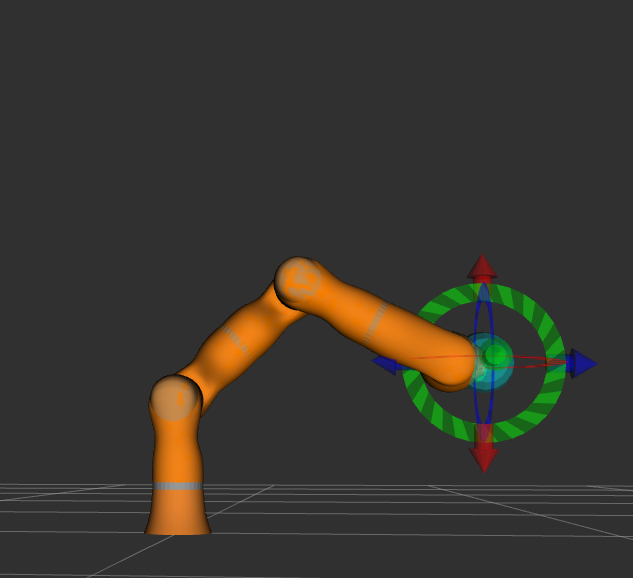
\includegraphics[width=1.20\textwidth]{images/kukaconfiguration2}
		\caption{Arm in non singular configuration}
		\label{nonsingular2}
	\end{minipage}
\end{figure}


\section{Evaluation on exploiting singularities}
The below table indicates the evaluation exploiting singular configurations. As discussed earlier, depending on the task performed by robot, there are two situations which are of concern. In cases of singular configurations, the indication is that the application of arbitrary external force on the end effector, does not produce any torque in the joints for the directions  of unsatisfiable task constraints i.e, in directions which the arm is singular.


\subsection{Experimental Setup}
The evaluation is conducted on two robot models KUKALWR4 and PUMA560. For KUKALWR4, the manipulator is maintained in home configuration with zero joint configuration (see fig \ref{singular1}). For PUMA560 is also maintained in home configuration, without including shoulder offset. The design of the kinematic chain follows the the joint specifications and frame assignments specified in OROCOS KDL. The models are also maintained to not compensate for gravity effects. 

\subsection{Results}
See \ref{exploit1} and \ref{exploit2} where the input external forces have been applied for all directions in the end effector. The only torques generated due to application of external forces is considered as the output resultant torque.
It can be seen that the there is no torque generated at all for certain directions of external forces. \color{blue}This indicates that, in that direction, application of arbitrary external forces results in torques in the joints which does not have any impact of external forces in them.\color{black}




\begin{table}[h!]
		\caption{Table indicating evaluation on exploiting singularities -PUMA560}
		\label{exploit1}
			\renewcommand{\arraystretch}{1.6}
			\resizebox{1.0\textwidth}{!}{%
	\begin{tabular}{|l|l|l|}
		\hline
		External force               & Resultant torques                            & Robot Model            \\ \hline
		linear x : {[}1,0,0,0,0,0{]}   & {[}-0.0064, -0.05079, -0.4318,0,0,0{]} & \multirow{6}{*}{PUMA560} \\ \cline{1-2}
		linear y : {[}0,1,0,0,0,0{]}  & {[}0.4318,0,0,0,0,0{]}                 &                          \\ \cline{1-2}
		linear z :  {[}0,0,1,0,0,0{]} & {[}0.0060, 0.4318, 0,0,0,0{]}          &                          \\ \cline{1-2}
		angular x : {[}0,0,0,1,0,0{]} & {[}0,0,0,0,0,0{]}                      &                          \\ \cline{1-2}
		angular y : {[}0,0,0,0,1,0{]} & {[}0.028, 0.227, 1.935,0,-1,0{]}       &                          \\ \cline{1-2}
		angular z: {[}0,0,0,0,0,1{]}  & {[}0,0,0,0,0,1{]}                      &                          \\ \hline
	\end{tabular}
}\renewcommand{\arraystretch}{2}
\end{table}


% Please add the following required packages to your document preamble:
% \usepackage{multirow}
\begin{table}[h!]
		\caption{Table indicating evaluation on exploiting singularities -KUKALWR4}
		\label{exploit2}
		\renewcommand{\arraystretch}{1.8}
		\resizebox{1.0\textwidth}{!}{%
	\begin{tabular}{|l|l|l|}
		\hline
		External force                & Resultant torques                               & Robot Model               \\ \hline
		linear x : {[}1,0,0,0,0,0{]}   & {[}7.9e-05,0.0887,0.00052,0.39,0,0,0{]}         & \multirow{6}{*}{KUKALWR4} \\ \cline{1-2}
		linear y : {[}0,1,0,0,0,0{]}  & {[}0,0,0,0,0,0,0{]}                             &                           \\ \cline{1-2}
		linear z :  {[}0,0,1,0,0,0{]} & {[}0,0,0,0,0,0,0{]}                             &                           \\ \cline{1-2}
		angular x : {[}0,0,0,1,0,0{]} & {[}0,0,0,0,0,0,0{]}                             &                           \\ \cline{1-2}
		angular y : {[}0,0,0,0,1,0{]} & {[}-0.0003,-0.379,-0.0022,-1.668,0.0026,-1,0{]} &                           \\ \cline{1-2}
		angular z: {[}0,0,0,0,0,1{]}  & {[}0,0,0,0,0,0,1{]}                             &                           \\ \hline
	\end{tabular}
}\renewcommand{\arraystretch}{2}
\end{table}

%will indicate that the drop in the rank of the matrix indicates singularity. Traditional singularity can be determined by calculating rank of the Jacobian. Similarly, 

%\subsection{Second scenario}
%For the second experimentation the 4 DOF model of the robot is developed in KDL. The mass of the segment was set to 1kg and length of the segment to 1 m. 
%\begin{itemize}
%	\item The initial configuration was set to be 
%\end{itemize}


\newpage
\section{Benchmarking on decompositions}
As discussed earlier in \cite{shakhimardanov2015composable}, the authors suggest the decomposition of rank one update as in \cite{sentana1999econometric} as a computationally less expensive decomposition than existing SVD. 


%The implementation is in python programming language
Measuring and analyzing the algorithm complexity aims at comparing different decomposition techniques and their rank one updates and their run time behaviors. The evaluation on the level of decompositions are necessary to measure the expensiveness of their operations. The efficiency of the algorithm depends on the time it takes to execute it completely which is based on the number of parameters used as input.


On analyzing the graphs \ref{svdvsrankone}, this graph performs a comparison of SVD decomposition and rank one update of LDL decomposition. The input parameters are varied for the number of constraints and number of segments. For the real time scenarios, it can be seen that the SVD performs better than the rank one update of LDL decomposition \cite{sentana1999econometric}. Similarly by comparing the run times for rank one update LDL decomposition, SVD and also the rank one update. It can be seen that SVD and rank one update of LDL decomposition has a linear relation for number of segments, and cubic relation on the number of constraints. But for rank one update on the LDL decomposition also shows a linear behaviour on number of segments and quadratic behavior on number of constraints.

%\ref{runtime-60}, it is seen that in real time scenarios SVD performs better than LDL rank one updates with linear complexity where the input parameter is the number of constraints. However, LDL rank one update performs better than SVD by introducing more number of constraints in the intermediate segments. In terms of numerical precision SVD is better. 



\begin{figure}[h!]
	\centering
	\begin{minipage}{0.45\textwidth}
		\centering
		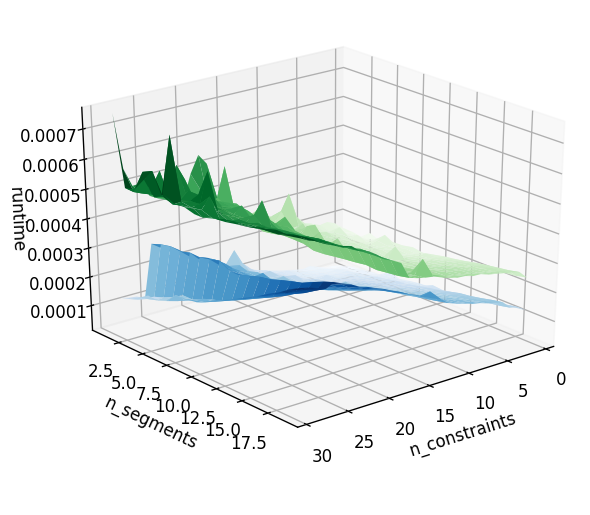
\includegraphics[width=1.0\textwidth]{images/svdvsrankone} % first figure itself
		\caption{Comparison of run time complexity for SVD and rankone update LDL}
		\label{svdvsrankone}
	\end{minipage}\hfill
	\begin{minipage}{0.45\textwidth}
		\centering
		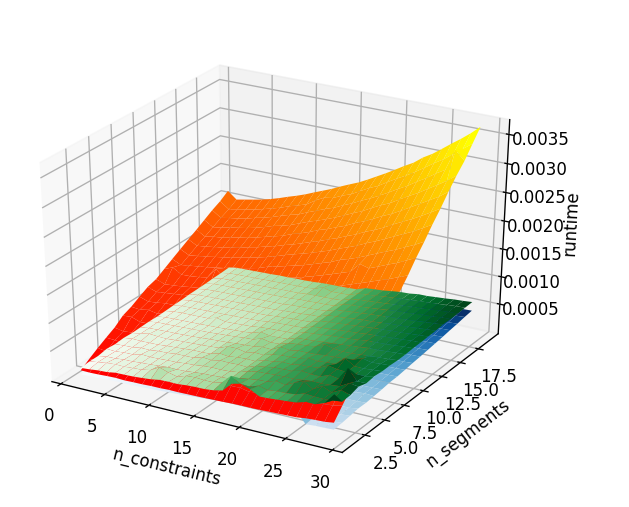
\includegraphics[width=1.0\textwidth]{images/all3} % second figure itself
		\caption{Situation depicting human carrying heavy box \cite{mot1}}
		{Case2: Necessity to utilize singular configuration}
	\end{minipage}
\end{figure}

\begin{figure}[h!]
	\centering
	\begin{minipage}{0.45\textwidth}
		\centering
		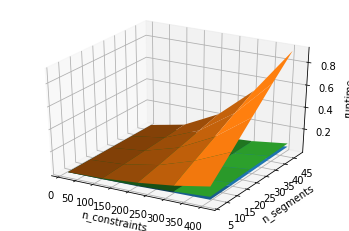
\includegraphics[width=1.0\textwidth]{images/plot3d1} % first figure itself
		\caption{Situation depicting robot carrying heavy tray \cite{robottray}}
		{Case1: Necessity to avoid singular configuration}
	\end{minipage}\hfill
	\begin{minipage}{0.45\textwidth}
		\centering
		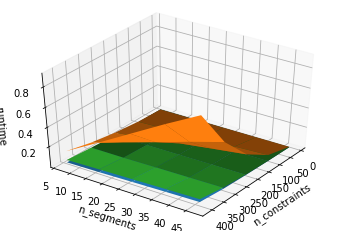
\includegraphics[width=1.0\textwidth]{images/plot3d2} % second figure itself
		\caption{Situation depicting human carrying heavy box \cite{mot1}}
		{Case2: Necessity to utilize singular configuration}
	\end{minipage}
\end{figure}
%
%		\begin{figure}[h!]
%			\centering
%			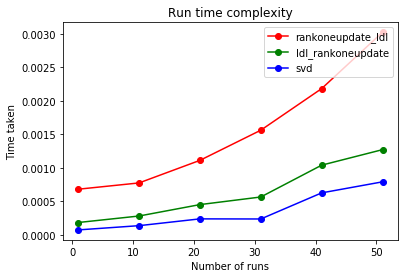
\includegraphics[width=0.5\textwidth]{images/n_60}
%			\caption{Run time complexity with number of constraints to be 60}
%			\label{runtime-60}
%		\end{figure}


%The run time complexity graph (see figure \ref{runtime}) is plotted for the number o.
%\begin{itemize}
%	\item Analyze with 4 different configurations - 2 in singular and 2 in not singular, valid in simulation as well. 
%	\item Jenny - with all joints in zero configuration, possible constraints, check while giving all constraints and then only achievable ones.
%	\item Inorder to measure the expensiveness of the operations involved in calculating the rank one updates in LDL and SVD. The comparison provides a benchmarking on run time performance. 
%
%	\item %Analyzing singularities in traditional approaches involve analyzing the Jacobians and rank of the Jacobian. In-order to evaluate the singularities occuring within the solver as mentioned in chapter \ref{} the constraint coupling matrix is analyzed.
%	\item As mentioned earlier, the analysed results are expected to involve losing rank of the matrices when the kinematic chain reaches singularity.
%	\item The experimental test setup included two major scenarios, one with the kinematic chain being in singularity and the other scenario 
%\end{itemize}

%\section{For Decomposition techniques}
%\begin{enumerate}
%\item {Run time performance}
%\item {Comparing different algorithms}
%\item {Numerical Robustness}
%\end{enumerate}
%\section{For singularities}
%Can you detect singularities?
%How do you know that robot is in singularity, traditional approach - ground truth, if jacobain loses rank then L also loses rank. Joint to jac solver, takes specification of kinematic chain, takes q returns jacobian for this robot in this configuration. svd and look at the sigmas.
%Which of the constraints can be satisfied?
%Can we detect during the sweeps?
%
%\section{Evaluation on test robot}
%-Not necessary - Consult Sven.
%\section{Cost- Expensiveness of particular motion}
%\section{Evaluation on level of physics}
%\begin{enumerate}
%\item Do your findings line up with classical singularities?
%\item Traditional approach considers velocities, how is it different in the solver? Acceleration - is it different?
%
%\item{Experimental Setup for singularity analysis}: 
%\item Are there singularities in which we can have velocities in particular direction but not acceleration?
%\item We are only looking into end effector accelerations.
%\item Singularity on velocity level and acceleration level are the same.
%
%\item Evaluation needs to be done on the level of energy domain which is an interesting point.
%\item Acceleration energy can it be linked to kinetic energy.
%\item Unit constrained force - f/m = a, f*a = accelenergy how are those related?
%\item tranformation between joint space and cartesian space with the inertia - kinetic energy level.
%\item When does jacobian lose rank in case of redundancy and why doesnt L matrix does not gain rank. Can we argue with forces, and for jacobian argue with velocities. How does jacobian to look like when two joints line up or the are being redundant- search, if my jacobian gets singular then my L matrix has to be singular should be the final argument.
%Two sources of singularity acceleration level and motion level.
%%$$\ddot(q) = J^{-1}^{ee} $$ "formula not complete"
%Jacobian if not full rank then cannot accelerate in particular direction, if there are more degrees of freedom than required then you have null space.
%Are they always singular at the same time, if so why?
%For L you are always adding rank, but for jacobians it always lose rank.
%S,D do not contribute to rank, it is mostly constraint forces, so by eqn 19, it shows that the constraint force of child element is projected and transformed.
%\item Transformation depends on q. J(q)= Jacobian depends on joint angles.
%When do you get singularity, in case where u cross a joint and you are not adding rank. 
%Compute the rank of Jacobian after u cross the first joint, it still remains the same rank, when two joints are redundant, similarly in L matrix.
%
%Now seeing eqn 15 and 16 linear inertia means how heavy does lifting the link and the whole kinematic chain. Articulated body inertia can not lose rank. There is no dynamic singularity in case of articulated inertia. Dynamic singularity is we are composing multiple projections and transformations together and they are not full rank.
%Now we see on the level of composing multiple projections and transformations together and they do not have full rank. This could be dual of classic singularities. 
%What does the projection do?
%What does the transformation of force do?
%two projections: projecting on joint axis, projection over joint axis.
%If there is no joint canceling out the force then it means it cannot produce movement in that direction. If you feel any end effector force at the base it means it cannot move in those directions. If you can accumulate the projections and transformations, it means it cannot move in those directions.
%Make an example on what does the projection mean.
%
%What of the constraint forces at the end effector do you feel at the base? If you feel any force at the base then it means that you cannot move in that direction.
%Take parents projection , transpose it and multiply with the base
%
%%Perform evaluation and benchmarking on the level of run time behaviour, write their complexities, refer audio lecture 13. and for LDL we have O(n.nc3) + O(nc2)(Base decomposition)  for SVD it is O(n.nc2) + O(nc3). In the realcase SVD seems to be better. What are the typical numbers that you have in there. If n is big then LDL, nc is big then SVD. big  mean around 1000. Kinematic chain in special situation where you have 10, 20. nc can be more for one segment upto 6. It looks like nc is almost constant. If you start introducing more constraints in the intermediate segments then more than 6, then this one give quickly expensive.What does O do it is eating up some constant factors,  SVD has rather big a in constant factors, whereas LDL has very small a. In terms of performance LDL is better. In terms of numerical precision SVD wins.  
%%SVD is usually numeric. 
%\end{enumerate}

%	\begin{figure}
%		\centering
%		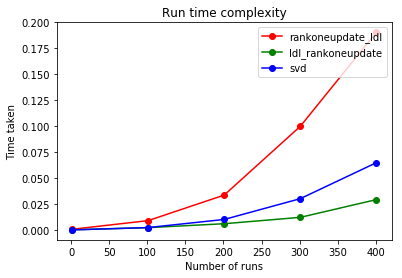
\includegraphics[width=0.5\textwidth]{images/runtimecomplexityn_500}
%		\caption{Run time complexity -nconstraints - 500}
%		\label{runtime}
%	\end{figure}

%\begin{itemize}
%	\item First explain KUKA LWR 3 cases test and validation. - Experimental setup, 3 cases of testing. - Theoretical explanation of why J loses rank and L loses rank.
%	\item Next Matrix Decomposition, run time graph explain complexity
%\end{itemize}
